%!TEX root = vmf_main.tex

\section{Application Examples}

\subsection{Piano Roll Visualization}

One method to quickly observe the general contour and structure of a piece of music is to visualize the music in a piano roll format. This is also a valuable tool for illustrating melodic contour and rhythmic composition to those who are unfamiliar with conventional music notation (an application of this type of representation is common in music and rhythm based video games). Music stored in the Vector Music Format can be easily converted to a piano roll graphical representation due to the structure of a VMF file.

One of the key features of the Vector Music Format is that every ``tick'' has the same temporal value. Because of this feature, it is best that the x-axis (time) uses ticks in increments of one unit. For the y-axis, as in all piano roll visualizations, a horizontal division should be used for each key on the piano keyboard. The lowest pitches are placed at the bottom of the y-axis and the highest pitches are placed at the top of the y-axis. This axis configuration allows the reader to easily view rhythmic structure by reading the visualization from left to right and to easily view melodic countour by reading the visualization in the vertical sense.

Once the two axes are properly prepared, the contents of the VMF body can be plotted by iterating through the tick vectors one by one. Within each tick vector, the same process is repeated for each of the parts or voices contained within. First the attack dimension must be evaluated: if the value is 0, then there is a silence at this tick and the next tick can be evaluated. If the value is 1, then a rectangular segment is opened at the current tick position for the pitch depicted by the pitch class and octave dimensions of the vector. Finally, if the value of the attack dimension is 2, then the note is being sustained from a previous tick and the rectangular segment which was previously opened is extended. If the last vector had a value of 2 in the attack dimension and it is followed by a vector with a value of 1, the rectangular segment is closed and a new one is opened at that position to indication a new note attack. If the last vector had a value of 2 in the attack dimension and it is followed by a vector with a value of 0, the rectangular segment is simply closed and silence (empty space) follows in the current tick. This behavior can be summarized in the extended finite state machine diagram in \ref{fig:visualizationStateMachine}. A Python implementation of this procedure is available at \href{https://github.com/project-schumann/vmf-visualization}{Github} illustrating how this visualization can be easily generated with a single traversal of a VMF file by using the ruls illustrated in the finite state machine presented in \ref{fig:visualizationStateMachine}. A piano roll visualization of the last movement of J.S. Bach's BWV 108 genedated by this script is shown in \ref{fig:bwv108PianoRoll}.

\begin{figure}
  \begin{center}
    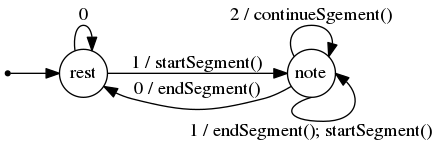
\includegraphics[scale=0.75]{resources/visualizationFSM}
    \caption{Visualization State Machine}
    \label{fig:visualizationStateMachine}
  \end{center}
\end{figure}

\begin{figure}
  \begin{center}
    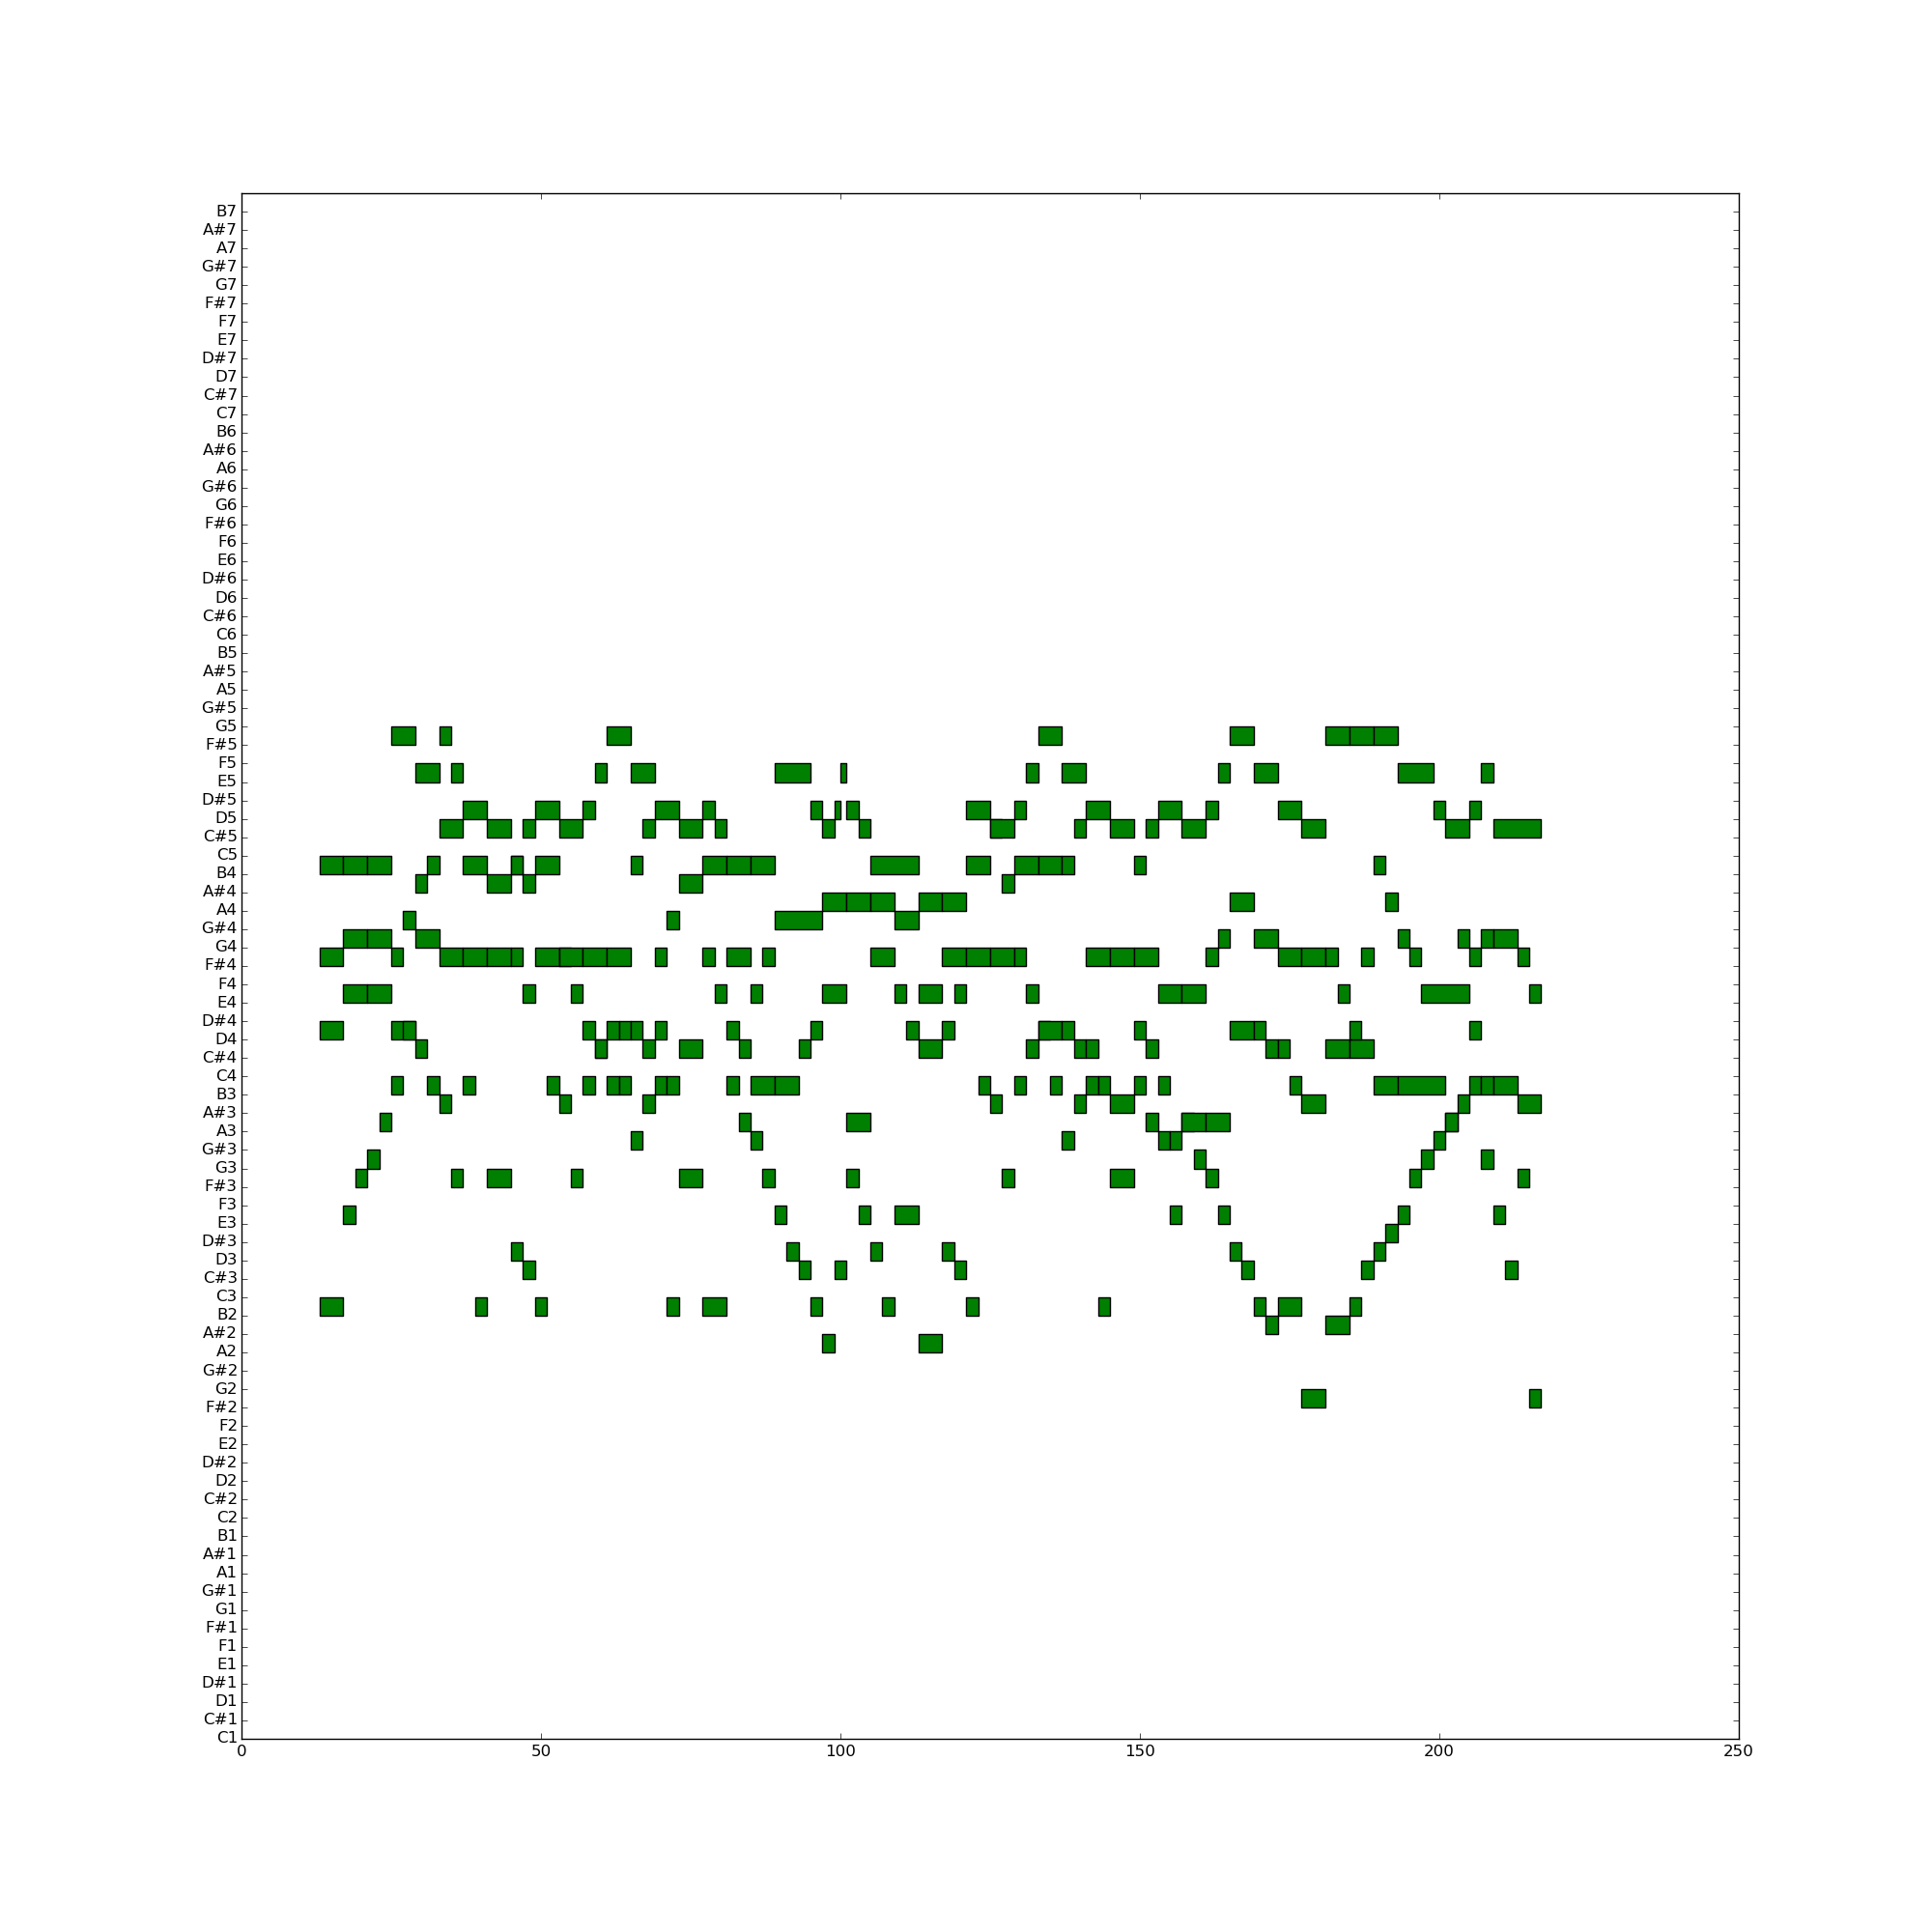
\includegraphics[scale=0.35]{resources/bwv108PianoRoll}
    \caption{Piano Roll Visualization of J.S. Bach BWV 108, Last Movement}
    \label{fig:bwv108PianoRoll}
  \end{center}
\end{figure}

When creating a visualization directly from a MIDI file, the algorithm used depends on the type of MIDI file used. As described in ``Beyond MIDI'' \citep*{HeSe97}, there are three possible types of MIDI files; format 0, format 1, and format 2. Format 0 restricts data to a single track, format 1, allows multiple independent melodic tracks which are all synchronized to a single time line, and format 2 allows tracks which are temporally independent. When dealing with a format 0 or format 1 MIDI file, constructing the visualization is similar to visualizing a VMF file by plotting notes on the timeline by observing the note-on and note-off MIDI messages. When dealing with format 2 MIDI files, some additional work is necessary to synchronize all tracks to the same time line before plotting notes on the timeline.

